\lstset{
  language=Idris, 
  morekeywords={->,=,:},
  backgroundcolor=\color{white},
  keywordstyle=\color{kw_orange},
  showtabs=false,     
  showspaces=false,                
  showstringspaces=false,             
  tabsize=2  
}
\subsection{Data Structures} \label{code_structs}
\subsubsection{The \inl{WeightOps} data type}
Our implementation of Dijkstra's algorithm allows user-defined edge weight type, with a \inl{WeightOps} data type specifying the operations and properties of the edge weight type that user needs to provide. \inl{WeightOps} is similar to a Java interface for the user-defined weight type, except that it also includes properties of the weight type besides the operators. 

Below presents part of the definition of \inl{WeightOps}. 
\begin{lstlisting}
      using (weight : type)
        record WeightOps weight where
          constructor MKWeight
          -- zero value of weight
          zero : weight
          -- greater than or equal to
          gtew : weight -> weight -> Bool
          -- equality
          eq : weight -> weight -> Bool
          -- addition
          add : weight -> weight -> weight
          ...
          triangle_ineq : (a : weight) -> 
                          (b : weight) -> 
                          gtew (add a b) a = True
          ...
          addComm : (a : weight) -> 
                    (b : weight) -> 
                    add a b = add b a
\end{lstlisting}

\inl{WeightOps} is defined as a record data type, which allows programmers to collect several values (referred as record's fields) together. \inl{WeightOps} is parameterized over the user-defined edge weight type \inl{weight}. The \inl{MKWeight} constructor takes in all the fields and build a \inl{WeightOps weight} type. The field name can be used to access the field value. For instance given a value \inl{ops} of \inl{WeightOps weight} type, \inl{add ops} will gives the addition operator for the \inl{weight} data type. 
\\

The \inl{zero} field stands for the zero value for the \inl{weight} type, and \inl{gtew, eq, add} are basic operators of \inl{weight}: \inl{gtew} is the greater than or equal comparator, \inl{eq} is the operator for checking equality, and \inl{add} is the operator for calculating addition. The \inl{triangle_ineq} field in \inl{WeightOps} ensures that the value of \inl{weight} data type can only be non-negative. Given any two values \inl{a, b} of type \inl{weight}, \inl{triangle_ineq} specifies that the sum of \inl{a, b} is greater than or equal to either of them, which guarantees that both \inl{a, b} have non-negative values. The remaining fields in \inl{WeightOps} are required for Dijkstra's implementation and verification, for instance the \inl{addComm} property (which states commutativity for the \inl{add} operator) is later applied in one of the helper functions in proving Lemma \ref{lemma4.1} in Section \ref{lemma1V}. 
\\

To provide a concrete example of constructing a \inl{WeightOps} data value, we present the definition of the \inl{natOps} variable below. 
\begin{lstlisting}
      -- a `WeightOps' for `Nat'
      natOps : WeightOps Nat
      natOps = MKWeight Z gte (==) plus
                        ...
                        nat_tri ... plusCommutative
\end{lstlisting}

We have eliminated a few fields in the definition of \inl{natOps} as they do not concern us here. The type of \inl{natOps} indicates that this record collects operators and properties for the \inl{Nat} data type. The first argument passed into \inl{MKWeight} for constructing \inl{natOps} is \inl{Z}, which is the zero value for \inl{Nat} and corresponds to the \inl{zero} field in the definition of \inl{WeightOps} data type. The next few arguments of \inl{MKWeight} provides the greater than or equal, equal, and plus operators for \inl{Nat}. The \inl{nat_tri} function states triangle inequality for \inl{Nat}, which ensures that the there is no negative values of the \inl{Nat} data type, and \inl{plusCommutative} is a built-in function in Idris that states commutativity for the \inl{plus} operator of \inl{Nat}. We can also define \inl{WeightOps} for other \inl{weight} types, for instance the \inl{Double} type, or even \inl{Char} type with user-defined operators for comparison, add, and checking equality etc., and the process of constructing \inl{WeightOps} data values over other \inl{weight} types is similar to the definition of \inl{natOps} variable provided above. 
\\

As we assume the input graph is a connected graph, the value of edge weight between two adjacent nodes are considered as not infinity, whereas Dijkstra's algorithm initializes the distance value from source node to all other nodes in the graph as infinity. Based on this consideration, we define a \texttt{Distance} type to represent the distance value between two nodes. \st{Distance} is parameterized over the user-defined \st{weight} type, and the value of \st{Distance weight} is either infinity, or sum of \st{weight}s. The definition of \st{Distance} data type is provided below. 
\begin{lstlisting}
      data Distance : Type -> Type where
        DInf : Distance weight
        DVal : (val : weight) -> Distance weight
\end{lstlisting}

The data constructor \st{DInf} builds a value of \st{Distance weight} that represents infinity distance, and \st{DVal} carries a value \st{val} of type \st{weight}, which is the sum of one or more \st{weight}s. Arithmetic operators for the \inl{Distance weight} type is defined based on operators of \inl{weight}.
\\

\subsubsection{Data Types for \inl{Node}, \inl{nodeset}, and \inl{Graph}} \label{graph}
The design of our data structures for a graph and its components are inspired by the adjacency list representation of a graph. We define the size of a graph as the number of the nodes in the graph. A graph of size \inl{gsize} is defined to contain a \inl{Vect} of \inl{gsize} \inl{nodeset}s, where \inl{nodeset} stands for the adjacent list for each node in the graph, and that each node in the graph carries the index for accessing its list of neighboring nodes from the graph. In other words, if we enumerate the set of nodes in a graph by natural numbers starting from 0, then the \inl{Vect} of \inl{nodeset}s is ordered in a sense that, the first element in this \inl{Vect} is the \inl{nodeset} for the node numbered 0, and the second element is the \inl{nodeset} for the node numbered as 1 ... etc. Figure \ref{figure2} illustrates this construction. 

\begin{figure}[H]
  \centering
  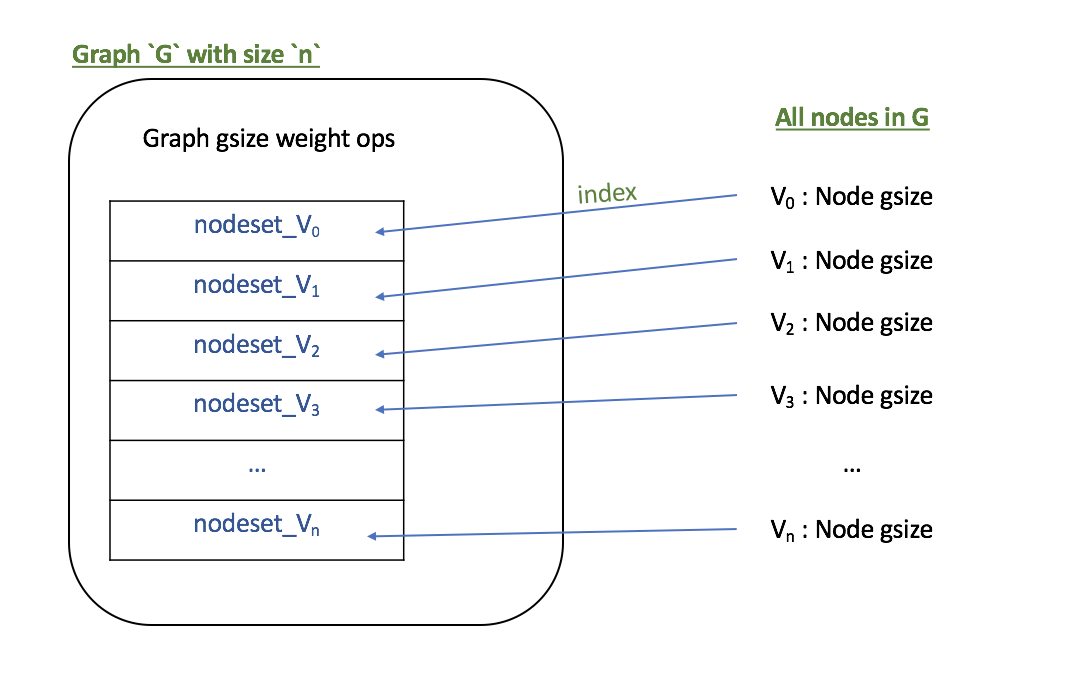
\includegraphics[scale = 0.6]{./figure/graphType.png}
  \caption{Graph Data Types Illustration}
  \label{figure2}
\end{figure}
\tab\\
The definition of \inl{Node}, \inl{nodeset} and \inl{Graph} data structure are presented below.

\begin{lstlisting}
      -- definition of Node
      data Node : (gsize : Nat) -> Type where
        MKNode : (nodeVal : Fin gsize) -> Node gsize

      -- definition of nodeset
      nodeset : (gsize : Nat) -> (weight : Type) -> Type
      nodeset gsize weight = List (Node gsize, weight)

      -- data type for Graph
      data Graph : Nat -> (w : Type) -> (WeightOps w)-> Type where
        MKGraph : (gsize : Nat) ->
                  (weight : Type) ->
                  (ops : WeightOps weight) ->
                  (edges : Vect gsize (nodeset gsize weight)) ->
                  Graph gsize weight ops
\end{lstlisting}

A \inl{nodeset} is a \inl{List} of pairs of type \inl{(Node gsize, weight)}, where the first element of the pair is the neighboring node, and the second element is the edge weight. For instance, if the \inl{nodeset} of a node \inl{v} in graph \inl{g} contains a pair \inl{(w, edge_w)}, this means node \inl{v} has an edge to \inl{w} in \inl{g}, with edge weight \inl{edge_w}. As the edge weight type is user defined, the \inl{Graph} data type is parameterized over the edge weight type \inl{weight}, and index by the size of the graph \inl{gsize}(which means there are \inl{gsize} nodes in this graph). Operators and properties of \inl{weight} are carried in the \inl{Graph} data type by the \inl{ops} parameter. \inl{edges} is a \inl{Vect} of {nodeset}s with length \inl{gsize}, as each node in the graph has its corresponding \inl{nodeset}. Since each node carries the index for accessing its \inl{nodeset} in the graph, a \inl{Node} type is indexed by the graph size \inl{gsize}, and defined to carry a value of type \inl{Fin gsize}. Relating to what we discussed above, to enumerate all nodes in the graph, the \inl{Node} numbered as 0 carries the value \inl{FZ}, and the \inl{Node} numbered as 1 carries the value \inl{(FS FZ)} ... etc.
\\

The type \inl{Fin gsize} captures the set of natural numbers within the range from 0(inclusive) to \inl{gsize}(exclusive), with size \inl{gsize}, which means that are only \inl{gsize} possible values of the type \inl{Fin gsize}. Such construction ensures that, for a graph \inl{G} of type \inl{`Graph gsize weight ops'} (graph size is \inl{gsize} and edge weight type is \inl{weight}), the type \inl{Node gsize} indicates that there are indeed \inl{gsize} number of nodes in the graph \inl{G}. More importantly, as our implementation uses the value carried by each \inl{Node} to index its \inl{nodeset} in the graph, as long as we restrict the type of each node in \inl{G} as \inl{Node gsize}, then the value carried by each node would have the type \inl{Fin gsize}, which is guaranteed to be a bounded index for the vector \inl{edges} in \inl{G}. 
\\

Based on the above construction, a node \inl{m} is considered as adjacent to a node \inl{n} in a graph \inl{g} if \inl{m} is in the \inl{nodeset} of \inl{n}. The definition of adjacent nodes is provided below. 
\begin{lstlisting}
      adj : (g : Graph gsize weight ops) ->
            (n, m : Node gsize) -> 
            Type
      adj g n m = (inNodeset m (getNeighbors g n) = True)
\end{lstlisting}

The \inl{getNeighbors} function takes in a graph \inl{g} and a node \inl{n}, and gets the \inl{nodeset} of \inl{n} in \inl{g}, and the \inl{inNodeset} function takes in a node and a \inl{nodeset}, and returns true if the input node is in the input nodeset, returns false otherwise. \inl{adj} is defined as a predicate on the input graph \inl{g} and two nodes \inl{m, n}. The type \inl{`adj g n m'} states that the node \inl{m} is adjacent to node \inl{n} in \inl{g} as \inl{m} is an element of the \inl{nodeset} of \inl{n} in \inl{g}. 
\\

\subsubsection{\inl{Path} and shortest \inl{Path}} \label{path}
A path in a graph is defined as a sequence of non-repeating nodes, where each two adjacent nodes have an edge in this graph. A path can contain only one node, as specified by the \inl{Unit} data constructor below, or multiple nodes, as the \inl{Cons} data constructor allows a new path to be constructed from an existing path. Specifically, given a path from node \inl{s} to \inl{v}, if \inl{n} is an adjacent to \inl{v} (\inl{adj g v n} specifies that there is an edge from \inl{v} to \inl{n} in the graph \inl{g}), then we can obtain a new path from \inl{s} to \inl{n} by appending the node \inl{n} to the end of the existing \inl{s}-to-\inl{v} path. 
\begin{lstlisting} 
      data Path : Node gsize ->
                  Node gsize ->
                  Graph gsize weight ops -> Type where
        Unit : (g : Graph gsize weight ops) ->
               (n : Node gsize) ->
               Path n n g
        Cons : Path s v g ->
               (n : Node gsize) ->
               (adj : adj g v n) ->
               Path s n g
\end{lstlisting}

To implement a shortest path in a graph, recall in section \ref{definitions}, we define the length of a path as the sum of the weights of all edges in the path, and define a shortest path as follows:
\\\\
\tab Denote $\Delta(s, v)$ as a shortest path from $s$ to $v$, and $\delta(v)$ as the length of $\Delta(s, v)$. $\Delta(s, v)$ must fulfill: 
\begin{center}
$\Delta(s, v) \in path(s, v)$ 
\\
and 
\\
$\forall p' \in path(s, v)$, $length(\Delta(s, v)) = \delta(v) \leq length(p')$
\end{center}

The above definition specifies that given a shortest path $\Delta(s, v)$, the length of $\Delta(s, v)$ is smaller than or equal to the length of any other $s-to-v$ path in the graph. We then provide the following implementation of shortest path based on the above definition. 

\begin{lstlisting}
      shortestPath : (g : Graph gsize weight ops) ->
                     (sp : Path s v g) ->
                     Type
      shortestPath g sp {ops} {v}
        = (lp : Path s v g) ->
          dgte ops (length lp) (length sp) = True
\end{lstlisting}

The statement stated by the return type of \inl{shortestPath} is highly similar to our mathematical definition of shortest path above. Specifically, given a graph \inl{g}, and a path \inl{sp} from node \inl{s} to \inl{v} in \inl{g}, the definition of \inl{shortestPath} specifies that, given any path \inl{lp} from \inl{s} to \inl{v} in \inl{g}, the length of \inl{lp} must be greater than or equal to the length of \inl{sp}. \inl{dgte} is the greater than or equal to operator for \inl{Distance} data type. 
\\

\subsubsection{The \inl{Column} data type} \label{column}
As we mentioned back in section \ref{pseudo}, our implementation viewed Dijkstra's algorithm as generating a matrix, where each column in the matrix represents one state of the algorithm, we define a \texttt{Column} data type for this purpose. The definition of \texttt{Column} type is provided below. 

\begin{lstlisting}
      data Column : (len : Nat) -> (g : Graph gsize weight ops) -> (src : Node gsize) -> Type where
        MKColumn : (g : Graph gsize weight ops) ->
                   (src : Node gsize) ->
                   (len : Nat) ->
                   (unexp : Vect len (Node gsize)) ->
                   (dist : Vect gsize (Distance weight)) ->
                   Column len g src

\end{lstlisting}

The \inl{Column} data type takes in the input graph \inl{g}, the source node \inl{src}, the number of unexplored nodes \inl{len}, which is also the length of \inl{unexp}, the vector of unexplored nodes. \inl{dist} is a \inl{Vect} of distance values from source for all nodes in the graph, with length \inl{gsize} as there are \inl{gsize} number of nodes in the graph. As discussed in Section \ref{first_layer}, the construction of \inl{dist} ensures that the elements are ordered the same way as \inl{edges} in the \inl{Graph} structure above, i.e., the first element in \inl{dist} is the distance of the \inl{Node} that carries \inl{FZ}, and the second element in \inl{dist} is the distance of the \inl{Node} that carries \inl{`FS FZ'} ... etc., hence we can again use the value carried by each \inl{Node} to index its corresponding distance value stored in the \inl{Column} with a \inl{nodeDistN} function, which is mentioned in the implementation of Lemma \ref{lemma4.2} in Section \inl{lemma2V}. The \inl{Column} type is indexed by the number of unexplored nodes. As Dijkstra's requires a source node for running the algorithm, the type \inl{Column} is also dependent on the input graph as well as the source node \inl{src}.
\\

Such definition of \texttt{Column} data type provides enough information for us to calculate a new column in the matrix, as the \inl{unexp} and \inl{dist} vectors provides enough information for calculating the current unexplored node with minimum distance value and generating the new distance vector with updated distance values for all nodes in the graph. Our implementation of Dijkstra's algorithm has a recursive structure, and generates a new \inl{Column} with one less unexplored node during each recursive call. With an input graph of size \texttt{gsize}, the first column should have length \texttt{gsize} as all nodes are unexplored, and the last column generated contains an empty vector for unexplored nodes, and a vector of the minimum value from source to all nodes in the graph. 
